\newpage
\section{Tests unitaires}

\begin{lstlisting}
/**
 * Function used to add a new question to the card
 * 
 * @param q The question that the user wishes to add to his card
 * 
 * @return true if added, false if not
 */
public boolean add( Question q )
{
    try
    {
        if ( q == null )
        {
            throw new NullPointerException();
        }
        if ( questions.contains( q ) )
        {
            throw new QuestionDoubleException();
        }
        if ( q.getTheme() != theme || !q.getAuthor().equalsIgnoreCase( author )
                || !q.getSubject().equalsIgnoreCase( subject ) )
        {
            throw new QuestionIncompatibleException();
        }
        if ( questions.size() == 4 )
        {
            throw new BasicCardOverMaxQuestionsException();
        }
        questions.add( q.clone() );
    }
    catch ( NullPointerException npe )
    {
        npe.printStackTrace();
        return false;
    }
    catch ( QuestionDoubleException qde )
    {
        qde.printStackTrace();
        return false;
    }
    catch ( QuestionIncompatibleException qie )
    {
        qie.printStackTrace();
        return false;
    }
    catch ( BasicCardOverMaxQuestionsException bcomqe )
    {
        bcomqe.printStackTrace();
        return false;
    }
    return true;
}
\end{lstlisting}

\begin{figure}[h]
	\centering
	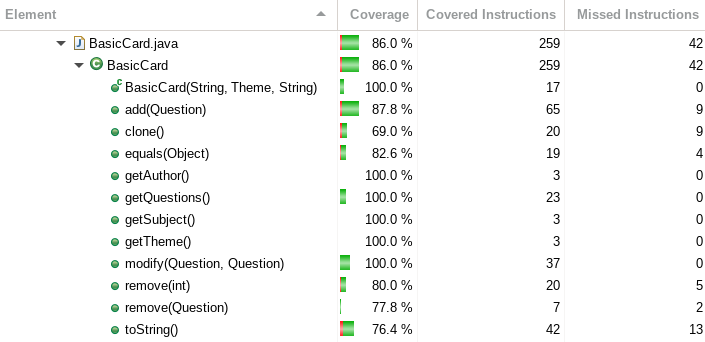
\includegraphics[width=\textwidth]{junit_coverage.png}
	\caption{Rapport de couverture du code}
	\label{fig:diag_coverage}
\end{figure}

